\section{Импульс тела}

\begin{center}
\begin{tblr}{
  colspec = {X[1.2,c]X[2,c]},
  vlines,
  hlines,
  row{1} = {font=\bfseries,mode=text},
  row{odd} = {bg=gray!10},
  cells = {mode=math,c,m},
  rowsep = 6pt
}
\text{Центр масс системы} & \text{Формулы и свойства} \\
\text{Определение} & \vec{R}_c = \dfrac{\sum m_i\vec{r}_i}{\sum m_i} \\
\text{Скорость системы} & \vec{V}_c = \dfrac{\diff\vec{R}}{\diff t} = \dfrac{\sum m_i\vec{v}_i}{\sum m_i} \\
\text{Импульс системы} & \vec{P}_c = M\vec{V}_c = \sum m_i\vec{v}_i
\end{tblr}
\end{center}

\begin{center}
\begin{tblr}{
  colspec = {X[1.2,l]X[1,c]},
  vlines,
  hlines,
  row{1} = {font=\bfseries,mode=text},
  row{odd} = {bg=gray!10},
  cells = {c,m},
  rowsep = 8pt,
  width = \textwidth
}
Уравнение Мещерского & Схема процессов массы \\
\parbox{0.5\textwidth}{
\centering
\large
$m(t)\dfrac{\diff\vec{v}}{\diff t}=\vec{u_1}\dfrac{\diff m_1}{\diff t}-\vec{u_2}\dfrac{\diff m_2}{\diff t}+\vec{F}$ \\
\normalsize
\begin{align*}
m(t) &- \text{мгновенная масса} \\
\vec{u_1} &= \vec{v}_1 - \vec{v} \quad \text{(отн. присоединение)} \\
\vec{u_2} &= \vec{v}_2 - \vec{v} \quad \text{(отн. выброс)} \\
\vec{F} &- \text{внешние силы}
\end{align*}
}
&
\begin{minipage}[c]{\linewidth}
\centering
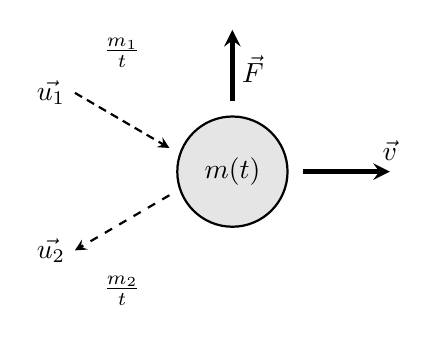
\begin{tikzpicture}[scale=1.0, >=stealth]
    % Основное тело с штриховкой для ч/б печати
    \draw[fill=black!10, thick] (0,0) circle (0.7);
    \node at (0,0) {$m(t)$};
    
    % Стрелка движения тела (сплошная толстая)
    \draw[->, ultra thick] (0.9,0) -- (2.0,0) node[above] {$\vec{v}$};
    
    % Присоединяемая масса (штрих-пунктир)
    \draw[->, thick, densely dashed] (-2.0,1.0) -- (-0.8,0.3);
    \node[left] at (-2.0,1.0) {$\vec{u_1}$};
    \node[above] at (-1.4,1.2) {$\frac{\diff m_1}{\diff t}$};
    
    % Отделяемая масса (пунктир)
    \draw[->, thick, dashed] (-0.8,-0.3) -- (-2.0,-1.0);
    \node[left] at (-2.0,-1.0) {$\vec{u_2}$};
    \node[below] at (-1.4,-1.2) {$\frac{\diff m_2}{\diff t}$};
    
    % Внешние силы (двойная линия)
    \draw[->, ultra thick] (0,0.9) -- (0,1.8);
    \node[right] at (0,1.3) {$\vec{F}$};
\end{tikzpicture}
\end{minipage}
\\
\end{tblr}
\end{center}